\chapter{Grundlagen der Ökologischen Nachhaltigkeit - Henk}
Zuallererst bedarf es einer Definitition der ökologischen Nachhaltigkeit und weshalb diese überhaupt erstrebenswert ist. Die Wirtschaftsweise der Menschheit ist stehts im Wandel und unterscheidet sich von Land zu Land. Die immer gravierender werdenden Auswirkungen des menschengemachten Klimawandels haben dazu geführt, dass in den Köpfen der meisten Einwohner der Industrieländer Gier und die ``Geiz ist geil'' Mentalität lange nicht mehr attraktiv sind. Auch vor dem Hintergrund von Finanz- und Weltwirtschaftskrisen scheint die Motivation für einen grundlegenden wirtschaftlichen Wandel sogar größer denn je. Sei es Elektromobilität, vegetarische oder vegane Ernährung, Fair-Trade-Produkte, Kooperation mit Hilfsorganisationen oder Energiewende, alles soll heutzutage 'nachhaltig' sein, doch was genau ist überhaupt mit Nachhaltigkeit gemeint? \newline Der Begriff Nachhaltigkeit geht in seiner Verwendung auf den Freiberger Oberberghauptmann Carl von Carlowitz (1645-1714) und die Waldwirtschaft zurück\cite{doi:nachhaltig}. Der Kern der Aussage, in der der Begriff vorkam, war, dass laut Carlowitz in einem Wald nur so viel abeholzt werden sollte, dass dieser stets über die Kraft verfüge, auf natürliche Art und Weise nachzuwachsen. Es ging also um eine schlaue Art der Waldbewirtschaftung, die es kommenden Generationen ermöglichen sollte, ebenfalls von der kontinuierlichen Nutzung des Waldes zu profitieren. Die Definition, die bis heute am meisten Anwendung sowie Anerkennung findet und um welche es in dieser Arbeit gehen soll, ist also, dass Nachhaltigkeit generell als die Fähigkeit definiert wird, die Bedürfnisse der heutigen Generation zu befriedigen, ohne die Möglichkeiten künftiger Generationen zu gefährden, deren Bedürfnisse ebenfalls zu befriedigen. \newline Nun bleibt zu klären, in welche Felder die Nachhaltigkeit aus wirtschaftlicher Perspektive gegliedert wird. Aus Abbildung 2.1 lässt sich entnehmen, dass die Nachhaltigkeit sowohl sozialer, ökologischer als auch ökonomischer Natur sein kann, ich werde mich aber nur auf die Ökologie fokussieren.\clearpage Die Grundlage unserer Existenz besteht aus natürlichen Ressourcen. Ob veganes Sojaschnitzel, Klamotten oder unser geliebtes Smartphone, für alle Produkte wurden Wasser, Böden und Rohstoffe genutzt. Ohne diese natürlichen Ressourcen wären wir heute nicht, wer wir sind. Diese Ressourcen sind jedoch begrenzt, gerade Rohstoffe wie Erdöl und Metalle werden irgendwann aufgebraucht sein und können nicht grenzenlos zu Produkten verarbeitet werden. Das gleiche gilt für Ressourcen wie Sauerstoff und Energie. Genau diese Umstände, dass Menschen und ihr Konsum eine Auswirkumg auf die Gesamtumweltsituation haben, fällt unter den Begriff der Ökologie. 
Umgangssprachlich wird das Adjektiv ``ökologisch'' als Ausdruck für eine Haltung oder ein Agieren verwendet, das schonend mit Umweltressourcen umgeht\cite[13-23]{test123}. Wie diese ökologische Nachhaltigkeit durch moderne Technologien wie einer Blockchain-Anwendung erreicht und unterstützt werden kann, soll im folgenden prognostiziert werden.

\begin{figure}[ht!]
	\centering
	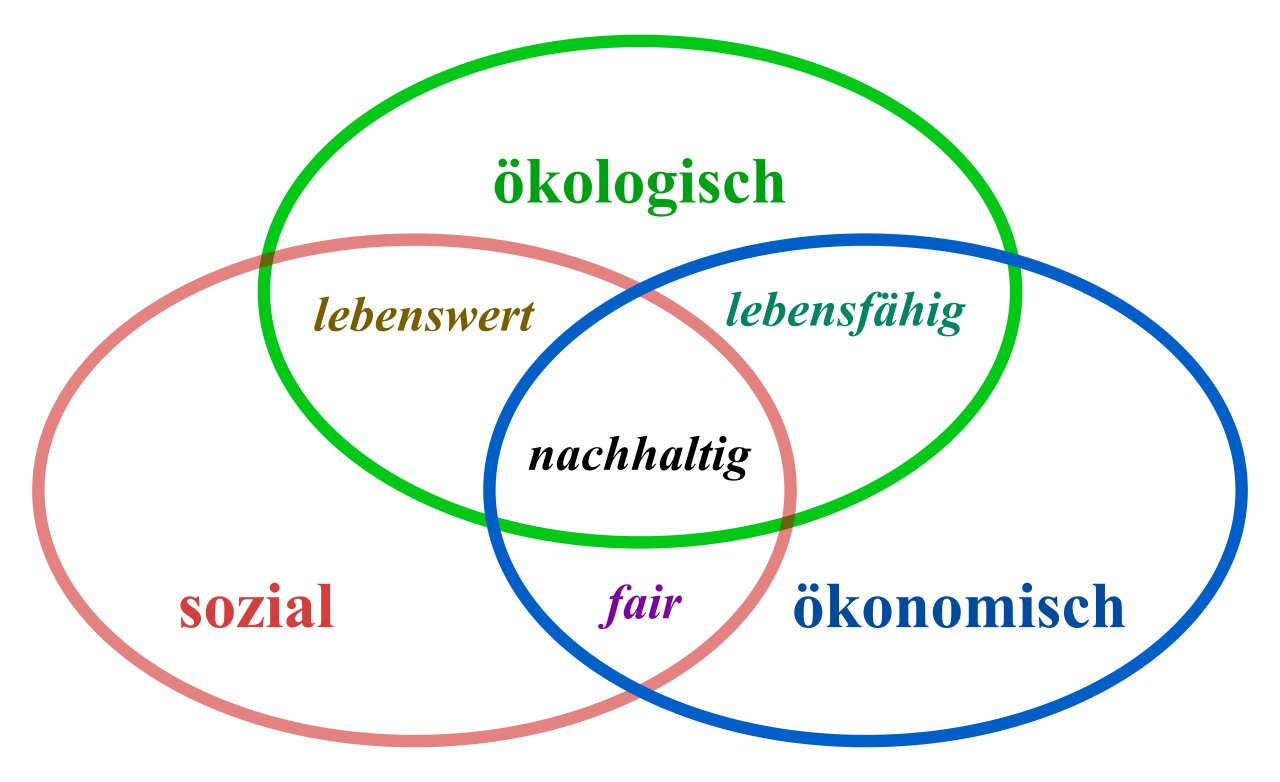
\includegraphics[width=100mm]{nachhaltig.jpg}
	\caption{Die drei Aspekte der Nachhaltigkeit\cite{oekologischeN} \label{overflow}}
\end{figure} 
\chapter{Technologische Grundlagen der Blockchain-Technologie}
\section{Mehr als nur Bitcoin - Nagi}
Beim Blick auf die Statistik wird ersichtlich, dass Bitcoin deutlich bekannter ist als die dahinter liegende Blockchaintechnologie \cite{Gbtcvsbc21}. Ohne die Blockchaintechnologie gäbe es die Kryptowährung Bitcoin nicht. Jedoch ist die Technologie für den Mainstream schwieriger greifbar als die Währung, die einige Menschen in kurzer Zeit reich gemacht hat. Sogar für Technickaffine ist es eine Herausforderung, Blockchain zu verstehen und zu erklären. Vor Allem die Öffentlichkeit präferiert es, über Dinge zu sprechen, die leichter verständlich sind. So etwas wie Blockhain, das schwierig greifbar oder gekauft %Was meinst du mit gekauft?
ist, ist kein wirklich gutes Thema für die Presse oder als Thema in unseren täglichen Gesprächen. Im Gegensatz dazu kann Bitcoin, das ebenfalls schwierig greifbar ist, zumindest online gekauft werden. Und die Presse kann aus Geschehnissen rund um den Bitcoin reißerische Schlagzeilen ziehen. Wie zum Beispiel: Dieser 18-jährige Teenager hat dank Bitcoin in 5 Jahren Milliarden von Dollar verdient \cite{Jeff18}, oder die Person, die nach diesem einen Computer sucht, auf dem er vor 10 Jahren einige Bitcoins geschürft (gemined) hat und ihn sehr reich machen würde, wenn er den Computer findet.
\newline 

All diese Art von Nachrichten tragen dazu bei, Bitcoin immer bekannter zu machen. Aber die Technologie hinter dieser Währung erfährt deutlich weniger Aufmerksamkeit. Das gleiche Konzept, das Bitcoin im Finanzbereich sehr erfolgreich gemacht hat, könnte jedoch in vielen anderen Bereichen eingesetzt werden und mehr Wert schaffen. Beispielsweise könnten die Energieauthentifizierung und die Stromversorgung (siehe Kapitel 4.4) viel transparenter und Strom dadurch billiger werden.  Auch im juristischen Sektor, der Medizintechnik oder der Verwaltung kann Blockchain verwendet werden, ohne Bitcoin zu nutzen.
(%Aber es braucht viel Zeit, um es zu erklären. Ich meine, es ist nicht so einfach, jemanden davon zu überzeugen, etwas Geld in Bitcoin zu investieren und in ein paar Tagen reich zu sein.)
Um diese alternativen Anwendungsmöglichkeiten der Blockchain nachzuvollziehen, ist es hilfreich, ein Grundverständnis für die Technologie zu entwicklen. Was ist also Blockchain: Eine Blockchain \cite{CW21} ermöglicht es, Informationen mithilfe einer dezentralen, von vielen Teilnehmern gemeinsam genutzten Datenbank fälschungssicher zu übermitteln, so dass Kopien ausgeschlossen sind. Die Datenbank wird auch als verteiltes Register oder Hauptbuch (Distributed Ledger) bezeichnet. Sie ist auf vielen Rechnern in einem Peer-to-Peer-Netzwerk abgelegt, wobei jeder neue Knoten mit seinem Beitritt eine vollständige Kopie der Blockchain übernimmt und ab sofort die Aufgabe hat, Transaktionen zu überprüfen und zu dokumentieren.
\section{Zentral vs Dezentral - Henk}
Um das benötigte Verständnis zu schaffen, werden wir einige Grundlagen über Blockchain und Kryptowährungen klären und kurz erläutern, in welchem Zustand sich aktuelle Internetanwendungen befinden und wie diese in Zukunft aussehen könnten. \newline

Die ersten Computernetzwerke entstanden in den 1960er Jahren. Über die folgenden drei Jahrzehnte entwickelte sich das Netzwerk, welches unter dem Namen ARPANET vom Verteidigungsministerium der Vereinigten Staaten begründet wurde, zum Internet, das wir heute kennen und täglich verwenden\cite{arpanet}. Weitere 30 Jahre nachdem das Internet massentauglich wurde, bilden zentrale Datenarchitekturen immernoch die Grundpfeiler des gesamten Netzwerks. Das heißt, unsere Daten werden zentralisiert auf wenige Computer, welche als Server im Netzwerk Kopien jener Daten speichern und bereitstellen, damit sie von für uns Nutzer oder Clients stehts abrufbereit sind. Diese Praktik sollte Misstrauen hervorrufen, denn wenige, mächtige Institutionen sind somit in der Lage, wenn sie es denn wöllten, sehr effizient Daten zu manipulieren, zu löschen oder aber nur bestimmten Nutzern den Zugriff zu erlauben. Dafür müssten sie in den meisten Fällen nur genau einen Punkt im Netzwerk kontrollieren.\cite{censorship} Betrachtet man die ganze Welt, wird man schnell fündig, wie manche Regierungen von besagter Macht kurzerhand Gebrauch machen. 2017 hat die spanische Regierung genau diese Problematik ausgenutzt, um die Unabhängigkeit der Katalanen zu verhindern\cite{catalonia}.
\clearpage

\begin{figure}[ht!]
	\centering
	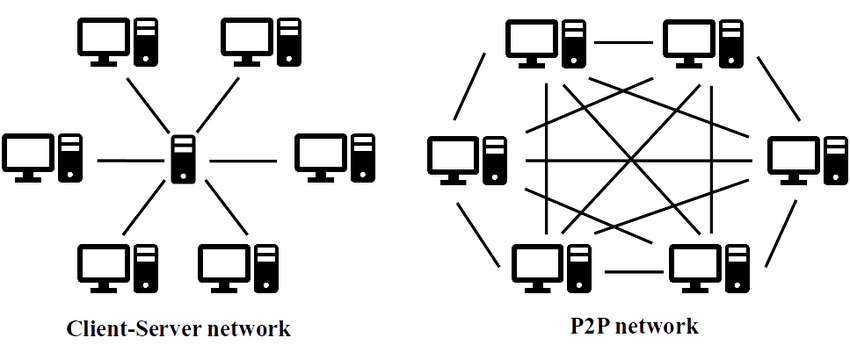
\includegraphics[width=100mm]{peer2peer.jpg}
	\caption{Vgl. Zentral vs. Dezentral\cite{p2p} \label{overflow}}
\end{figure} Eine alternative Architektur ist die der Dezentralität. Diese dezentralen Anwendungen basieren auf sogenannten Peer-to-Peer-Netzwerken, in denen die Benutzer untereinander direkt kommunizieren und dies eben nicht über einen sich in der Mitte befindenden Server tun. Anwendungen dieser Art gibt es nicht erst seit 2009, dem Jahr in dem der Bitcoin vorgestellt wurde, aber mit ihm wurde ein neues Prinzip erfunden, das es anonymen Teilnehmern eines riesigen globalen Netzwerks ermöglicht, ein gegenseitiges Vertrauen zu schaffen, welches zuvor nur durch juristisch bindende Verträge oder zentrale Institutionen, also Banken oder Plattformen wie Google und Facebook, geschaffen werden konnte. Die Grundlage des Bitcoin-Protokolls ist, dass alle aktiven Teilnehmer, auch Nodes genannt, lokal eine Kopie des gemeinsamen Kursbuches (im Englischen ledger) abspeichern, wie es sonst nur von Banken geführt wird. In diesem Kursbuch stehen alle bisher getätigten Transaktionen seit Beginn des Bitcoins. Der Unterschied ist, dass in diesem Fall nicht ein zentraler Akteur eine einzige Kopie des Ledgers besitzt, sondern gleich alle Akteure weltweit Kopien mitführen. Es handelt sich also um ein verteiltes Kursbuch bzw im Englischen einen ``distributed ledger''. Das Bitcoin-Netzwerk wird auf den Händen dieser besagten Nodes getragen. Wollen diese Nodes aktiv neue Transaktionen ins Kursbuch hineinschreiben, so müssen sie im Bitcoin-Protokoll einen Beweis darüber vorzeigen, dass sie eine gewisse Rechenleistung erbracht haben, den sogenanngen Proof of Work. Hierdurch entsteht die Sicherheit des gesamten Netzwerks. Die verarbeiteten Transaktionen werden anschließend in Blöcke zusammengefasst und als Paket in das Kursbuch eingefügt. Es handelt sich also um eine immer länger werdende Kette aus Blöcken, daher der Begriff Blockchain. Für jeden Block, den ein Miner, also jemand der eine Node betreibt um neue Blöcke zu erstellen, an die Kette anfügt, wird er wiederum mit Bitcoins belohnt, dafür dass er für die Sicherheit des Systems sorgt. \cite{bitcoinWiki}\cite{tokenEco}. \newline
\section{Smart Contracts als Grundlage für Anwendung auf der Blockchain - Nagi}



Ein Smart Contract \cite{CW18} ist ein Computercode, der die Ausführung bestimmter vertraglicher Vereinbarungen vereinfacht, indem er die Notwendigkeit eines Vermittlers überflüssig macht. Smart Contracts sind eng mit der Blockchain-Technologie verknüpft, da diese die Plattform ist, auf der sie basieren. Mit anderen Worten, Smart Contracts befinden sich in der Blockchain. Es gibt unzählige auf Smart Contracts basierende Anwendungen und viele Einsatzmöglichkeiten.

Lieferdienste sind ein Beispiel für eine Aktivität, bei der Smart Contracts leicht angewendet werden könnten. Ein Smart Contract würde sicherstellen, dass das Geld erst nach der tatsächlichen Zustellung des Pakets an den Lieferdienst gesendet wird. Es ist nicht mehr notwendig, einen traditionellen Vertrag zu unterzeichnen; der Absender füllt den Smart Contract einfach mit einer Kryptowährung aus, dann verwendet der Smart Contract die Währung (Bitcoin kann ein Beispiel sein), um alles abzuwickeln.

Mit anderen Worten, ein Smart Contract führt das aus, was in seinem Code geschrieben ist, solange bestimmte Bedingungen erfüllt sind. Das macht Transaktionen transparent, manipulationssicher, schnell und irreversibel. Darüber hinaus ist die Anwesenheit einer zentralen Behörde nicht erforderlich. Es ist einfach ein Code, der zwei Parteien hilft, ohne Zwischenhändler zusammenzuarbeiten.
Das Konzept der Smart Contracts gibt es seit über zwanzig Jahren, aber erst mit dem Aufkommen der Blockchain wurde es in großem Umfang eingesetzt.

Smart Contracts können für den Austausch von Geld, Waren oder anderen Vermögenswerten sehr praktisch sein, was dazu beiträgt, Geschäftsprozesse zu rationalisieren und Wartezeiten für die Validierung, die Rückverfolgung von Lagerbeständen, die Automatisierung von Dividendenzahlungen oder die Kontrolle personenbezogener Daten zu vermeiden. Sie können in den Bereichen Finanzen, Energie, Immobilien, Gesundheitswesen, Medien, Unterhaltung und Regierung eingesetzt werden.

Es wird erwartet, dass die Nachfrage nach Smart Contracts im Zusammenhang mit der Entwicklung des Internets der Dinge (IoT) zunehmen wird. Darüber hinaus sind Smart Contracts und ICOs eng miteinander verknüpft, da letztere Smart Contracts verwenden, um den Währungsaustausch zu erleichtern.

Allerdings stehen Smart Contracts erst am Anfang und es gibt noch viele Fragen, die angegangen werden müssen, angefangen bei der Sicherheit. Stellen Sie sich einen Smart Contract vor, der große Sicherheitslücken aufweist, aber nicht schnell behoben werden kann ... Es gibt auch Fragen der Regulierung und die rechtlichen Aspekte von Smart Contracts.

Ethereum Smart Contracts sind die beliebtesten.

\section{Konsensalgorithmus - Nagi}

Laut Binance Academy ist Ein Konsens-Algorithmus ein Mechanismus, der es Benutzern oder Maschinen ermöglicht, sich in einer verteilten Umgebung zu koordinieren. Er muss sicherstellen, dass sich alle Agenten im System auf eine einzige Quelle der Wahrheit einigen können, selbst wenn einige Agenten versagen. Mit anderen Worten, das System muss fehlertolerant sein. \cite{Binance21}
\newline
Da Blockchain dezentral funktioniert und großvolumige Transaktionen in Echtzeit aufzeichnet, kann die Komplexität der Wahrheit bestehen. Der Schlüssel besteht darin, auf die eine oder andere Weise einen Konsens zu erzielen, da sonst böswillige Dinge wie Double-Spend-Angriffe auftreten können. Hier kommt der Konsensalgorithmus ins Spiel.


Für Blockchain-Netzwerke sind die Konsensalgorithmen ein wesentliches Element, da sie die Integrität und Sicherheit dieser verteilten Computersysteme aufrechterhalten. Die beiden Haupttypen dieses Algorithmus sind Proof of Work und Proof of Stake. Und dieses Bild erklärt sie beide.

\begin{figure}[ht!]
	\centering
	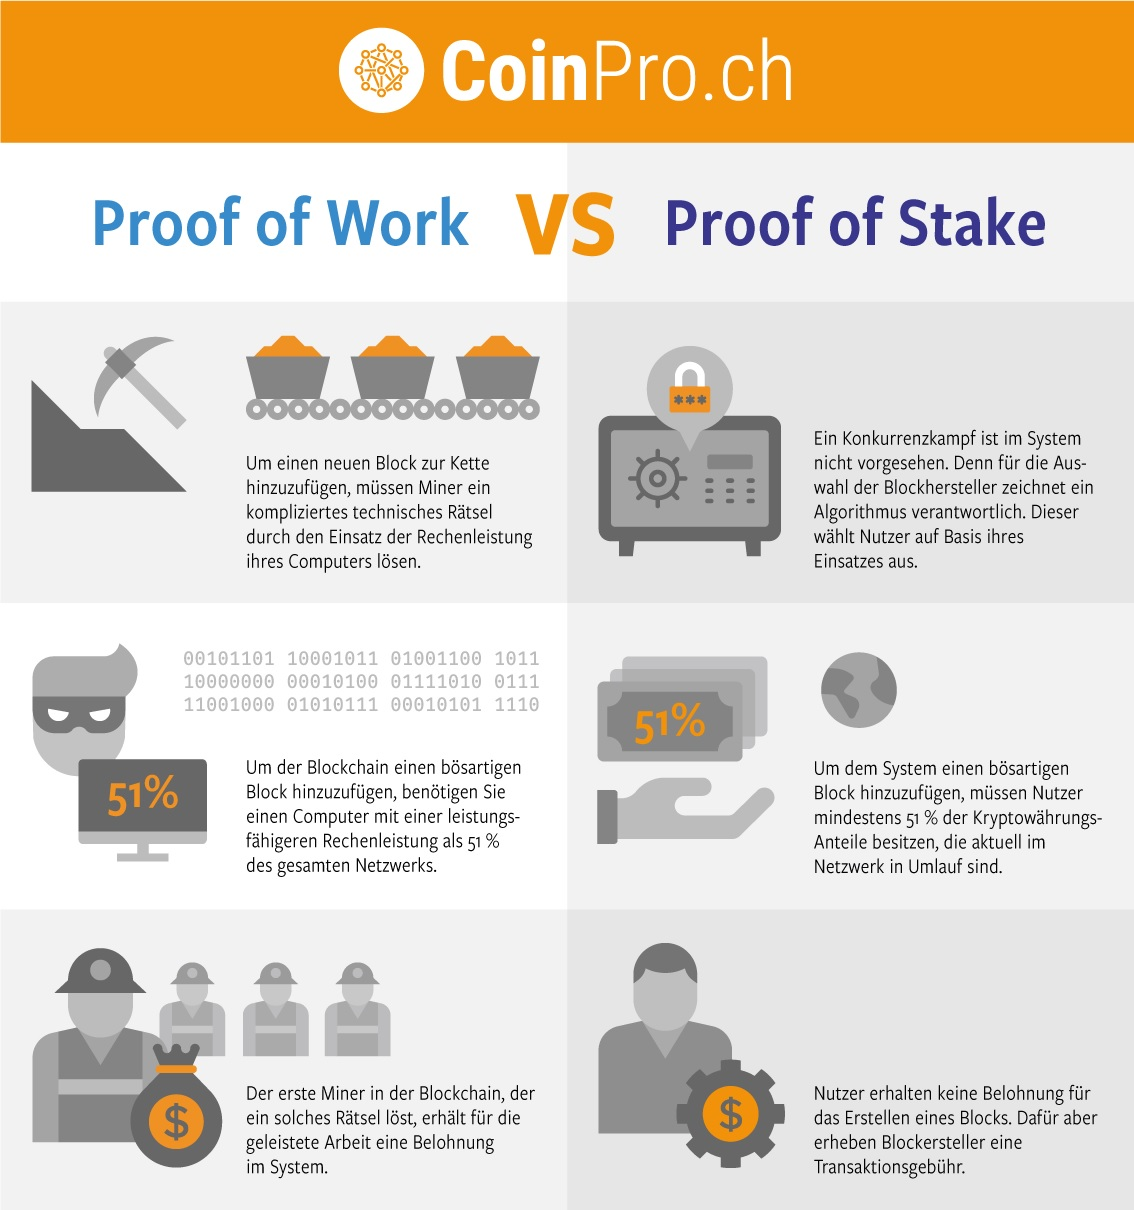
\includegraphics[width=160mm]{ProofOfWorkVSProfOfStake.jpg}
	\caption{Infografik zu den Unterschieden von Proof of Work und Proof of Stake} \label{overflow}
\end{figure}

\chapter{Chancen und Risiken}
\section{Risiko - CO2-Emissionen durch Kryptowährungen - Samuel}
Eine populäre Anwendung der Blockchaintechnologie sind Kryptowährungen, wie zum Beispiel Bitcoin \cite{schinckus_good_2020}. Die Nachfrage nach Bitcoin - und entsprechend sein Preis - ist über die letzten Jahre, aber vor Allem seit Oktober 2020, stark angestiegen. Somit betrug der Preis für einen Bitcoin zwischenzeitlich über 60.000 USD \cite{noauthor_coindesk_2021}. Doch im Mai 2021 stürzte der Kurs um bis zu 50\% ab. Einer der Gründe war die Ankündigung von Tesla CEO Elon Musk, dass der Autobauer mit sofortiger Wirkung keine Zahlungen mehr in Bitcoin akzeptieren würde. Motivation für die Maßnahme seien die Bedenken zur Umweltunverträglichkeit der Technologie hinter Bitcoin \cite{waters_musk_2021}. 

Dieses Kapitel skizziert diese Technologie und erläutert negative Auswirkungen von Bitcoin auf die Umwelt und das Klima. \newline
Der von der Bitcoin-Blockchain genutzte Konsensalgorithmus (siehe Kapitel 3.4) ist der Proof-of-Work (POW) Algorithmus, welcher laut \cite{andoni_blockchain_2019} in ca. 60\% aller Blockchainapplikationen angewendet wird.  In POW validieren die Betreiber von Nodes, sogenannte „Miner“ Transaktionen innerhalb der Blockchain, indem sie den nächsten Block der Chain (Kette) finden und hinzufügen. Dafür müssen sie mithilfe von großer Rechenleistung einen Hash-Wert errechnen, der wiederum von anderen Teilnehmern des Netzwerks (nodes) bestätigt werden muss. Der erste Miner, der den Hash-Wert des neuen Blocks findet, wird im Falle der Bitcoin-Blockchain mit Bitcoin belohnt. Er hat somit einen Bitcoin „gemined“ (geschürft) \cite{adam_konsensmodelle_2020}. Jede 210.000 gelösten Blocks sinkt die Belohnung für die Miner um 50\% („Halving“). Während im Geburtsjahr des Bitcoin, 2009 noch 50 Bitcoin pro gelöstem Block ausgegeben wurden, sind es in 2021 noch 6,25. Dieses Verfahren sorgt für eine immer geringere Menge an neu ausgegebenen Bitcoins und wird sich solange fortsetzen, bis alle verfügbaren 21 Millionen Bitcoins „gemined“ sind \cite{schar_understanding_2020}. \newline

POW gilt, solange nicht mehr als 50\% der Rechenleistung im Netzwerk von einem Mining-Pool (ein Zusammenschluss von Minern) ausgehen, allgemein als sehr sicher \cite{gervais_security_2016}. Gleichzeitig ist der beschriebene Prozess des Minings aufwendig und bedarf das Lösen immer komplexer werdender Rechenaufgaben \cite{stoll_carbon_2019}\cite{schinckus_good_2020}. Dafür werden Computerprozessoren benötigt, die wiederum Strom konsumieren. Der Verbrauch hängt von der Effizient der benutzten Hardware ab. Es existieren verschiedene Studien mit verschiedenen Ansätzen zu dem geschätzten Stromverbrauch des gesamten Bitcoin-Netzwerks und den dabei verursachten CO2-Emissionen. \newline

	Calvo-Pardo et al. \cite{calvo-pardo_machine_2020} schätzen den CO2-Fußabdruck von Bitcoin in 2018 auf 23,83 und 2019 auf 19,83 Mt. Eine andere Studie von Stoll et al. \cite{stoll_carbon_2019} kommt zu einem ähnlichen Ergebnis. Die Autoren basieren ihre Berechnungen jedoch auf mehr empirischen Daten, weshalb auf diese Studie gesondert eingegangen wird. Die Autoren argumentieren wie folgt: Durch das Halving lohnt es sich aus ökonomischer Sicht nicht mehr, handelsübliche Hardware für das Mining von Bitcoin zu nutzen. Solche Hardware ist zu ineffizient und würde durch den Stromverbrauch zumeist höhere Kosten verursachen, als sich beim Mining verdienen ließe. Stattdessen greifen Miner zumeist auf dezidierte Hardware von spezialisierten Herstellern wie Bitmain, Canaan oder Ebang zurück \cite{stoll_carbon_2019}. Basierend auf den Verkaufszahlen der drei Unternehmen schlussfolgern Stoll et al. (2019), dass ihre Hardware jeweils 78\%, 13\% und 9\% der Rechenleistung des Bitcoin Netzwerks abdecken. Darauf basierend wurde der minimale jährliche Stromverbrauch des Netzwerks berechnet. Für die Berechnung des maximalen Stromverbrauchs wurde davon ausgegangen, dass Miner zu jedem Zeitpunkt die ineffizienteste Hardware nutzen, die ihnen basierend auf dem aktuellen Bitcoin-Preis und einem durchschnittlichen Strompreis von 0.05 USD pro kWh eine Kostendeckung ermöglicht. Im Durchschnitt gehen die Autoren in 2018 von einem jährlichen Stromverbrauch von 45,8 TWh. Um wiederum den mit der benötigten Stromerzeugung verbunden CO2-Ausstoß zu berechnen, wurden die IP-Adressen von Pool-Servern und Endgeräten lokalisiert. Anschließend wurde der jeweilige regionale Strommix als Basis für eine Schätzung der verbundenden Kohlenstoffdioxidemissionen genutzt \cite{stoll_carbon_2019}. Stoll et al. \cite{stoll_carbon_2019} kommen so zu dem Ergebnis, dass die jährlichen CO2-Emissionen 22 – 22,9 MtCO2 betragen. Es ist anzumerken, dass der Preis für einen Bitcoin zum Zeitpunkt der Veröffentlichung der Studie von Stoll et al. \cite{stoll_carbon_2019} bei 10.500 USD lag \cite{noauthor_coindesk_2021}. Dieser hat sich aber seitdem vervielfacht, sodass sich die Frage stellt, ob der maximale Stromverbrauch entsprechend auch weit höher liegen könnte. Der Cambridge Bitcoin Electricity Index geht zum Zeitpunkt der Veröffentlichung der Studie von Stoll et al. \cite{stoll_carbon_2019} von einem Bitcoin Energieverbrauch von um die 50 TWh aus. Bis heute (Juni 2021) hat sich die Schätzung des Canmbridge Centre for Alternative Finance (CCAF) auf 117 TWh erhöht \cite{cambridge_cambridge_2021}. Basierend auf den geographischen Analysen von Stoll et al. (2019) und den damit einhegenden Kalkulationen zum CO2-Ausstoß und den aktuellsten Zahlen des CCAF könnten die Emissionen von Bitcoin heute 56,2 – 58,5 MtCO2 betragen (0,4803 bzw. 0,5 MtCO2 pro TWh). Bitcoin könnte also für ca. 0,18\% der globalen CO2 Emissionen von 31,5 Gigatonnen (=31.500 Mt) \cite{IEA_global_2021} verantwortlich sein. \newline
	
		Den hohen Stromverbrauch von Bitcoin mit erneuerbaren Energieträgern zu decken scheint dabei nur eine begrenzte Lösung zu sein, da Miner unabhängig von dem schwankenden Stromangebot erneuerbarer Energiequellen eine durchweg hohe Nachfrage \cite{de_vries_renewable_2019}. Diese kann zu dem Erhalt oder sogar zum Bau neuer Kohlekraftwerke, vor Allem in China, führen. Dies gilt nicht ausschließlich für Bitcoin, sondern auch andere, auf POW basierende Kryptowährungen, die Schätzungen zufolge etwa 50\% der Menge der Klimagasemissionen von Bitcoin verursachen \cite{gallersdorfer_energy_2020}. Ein Blick auf den angewandten Konsensalgorithmus könnte Wege zu niedrigeren Emissionen durch Kryptowährungen aufzeigen \cite{de_vries_renewable_2019}\cite{schinckus_good_2020}. \newline
		Neben dem von Bitcoin genutzten Konsensalgorithmus POW existiert auch das Proof-of-Stake (POS) Verfahren. In diesem Verfahren wählt das Netzwerk zufällig einen Forger (zu Deutsch: Schmied) – das Äquivalent zum Miner in POW - , der eine Transaktion bestätigen oder ablehnen kann. Als Sicherheitsmechanismus muss der Forger seine gehaltenen Anteile (Stake) als Kaution in Form der Kryptowährung im Netzwerk hinterlegen, die er nur zurückbekommt, wenn er Transaktionen nicht fälschlicherweise bestätigt oder ablehnt. Für jede Validierung erhält er außerdem eine Belohnung. Je größer der hinterlegte Anteil ist, desto wahrscheinlicher wählt das Netzwerk den Forger für eine Transaktionsvalidierung aus. POS wird deshalb teilweise kritisiert, wohlhabende Teilnehmer des Netzwerks noch wohlhabender zu machen. Andererseits bedarf ist für den Validierungsprozess keiner extra Hardware – dieser ist entsprechend deutlich weniger energieintensiv als bei POW \cite{adam_konsensmodelle_2020}\cite{schinckus_good_2020}. 
\section{Risiko - Entstehung von Elektromüll - Niels}

Wenn man sich mit der ökologischen Nachhaltigkeit von Blockchain auseinandersetzt, findet man viele Berichte über dessen Energieverbrauch. Dieser wurde im vorherigen Kapitel bereits behandelt und soll hier nur kurz angeschnitten werden. Im Anwendungsfall der Kryptowährung Bitcoin wird laut einer aktuellen schätzenden Statistik \cite{de_vries_bitcoin_nodate} jährlich 121,51 Terawattstunden an Energie verbraucht, damit die Geräte des Netzwerkes ihre Berechnungen des SHA-256 Hashes durchführen können. Die Hardware, welche für diesen Prozess des Schürfen (engl. Mining) verwendet wird, hat seit dem Beginn von Bitcoin vier Phasen \cite{taylor_evolution_2017} durchlaufen.
\newline
Zu Beginn wurde für das Schürfen die CPU verwendet. Ein optimiertes Modell wie das „Intel Core i7-990x“ konnte bis 33 Megahashes pro Sekunde berechnen. Diese Hardware ist allerdings für den allgemeinen Gebrauch gedacht und besitzt deshalb auch ein breites Spektrum an Optimierungen für nicht, in diesem Szenario, benötigte Operationen. Durch die Leistungseinbußen aufgrund der anderweitigen Optimierungen wurde der Fokus im Jahr 2010 auf GPU’s gelegt. Da Grafikkarten bereits eine bessere Optimierung für die notwendigen mathematischen Berechnungen hatten, ließen sich mit ihnen bis zu 675 Megahashes pro Sekunde berechnen. Somit haben sie bis zu 20 Mal mehr Arbeit verrichten können.
\newline
Der Nachfolger der Grafikkarte kam bereits ein Jahr später und dabei handelte es sich um FPGA’s. Die Bezeichnung FPGA steht für „Field Programmable Gate Array“ und bezeichnet dabei ein Gerät, mit dem sich digital benutzerdefinierte Schaltkreise darstellen lassen, welche einen viel höheren Grad der Optimierung zuließen. Dies äußerte sich nicht in der Menge der Hashwerte, welche sie pro Sekunde berechnen konnten, sondern auch durch ihre Energieeffizienz. Ihr Nachfolger und die aktuelle bevorzugte Geräteart sind ASIC’s, dabei steht die Abkürzung für „Application Specific Integrated Circuit”. Sie bieten nochmals einen höheren Grad der Optimierung als FPGA’s an. Besitzen allerdings den Nachteil, dass die Schaltkreise sich nach dem Fertigungsprozess nicht mehr anderweitig programmieren lassen. Eines der ersten Geräte konnte bis zu 60 Gigahashes pro Sekunde berechnen und war damit bereits 100 Mal schneller als seine Grafikkarten oder FPGA Konkurrenten. Ab diesen Zeitpunkt  war es ein Wettkampf der ASIC-Hersteller, wer die energieeffizientesten Geräte anbieten konnte. Zur Zeit ist das leistungsstärkste und energieeffizienteste Gerät der „Antminer S19 Pro“ \cite{michel_rauchs_cbeci_nodate} von Bitmain mit 110 Terahashes pro Sekunde.
\newline
Wie bei dem Stromverbrauch lässt sich nicht genau festlegen, wie viele Geräte aktive am Bitcoin Netzwerk arbeiten. Es ist aber möglich eine Schätzung anhand der aktuellen Hashwertrate \cite{blockchaincom_statistic_nodate} des Netzwerkes zu geben. Laut dem Stand vom 31 Mai 2021 wurden pro Sekunde 150,292 Millionen Terahashes berechnet. Wenn nun angenommen wird das im gesamten Netzwerk nur eine Art von Gerät verwendet wird, wie beispielsweise der „Antminer S19 Pro“, lässt das den Schluss zu das ungefähr 1,366 Millionen Geräte benötigt werden um diese Rechenleistung zu erreichen. Der „Antminer S19 Pro“ wiegt nun 13,2 kg was in der Masse ein Gewicht von 18,0312 Kilotonnen ergibt. Wie Alex de Vires \cite{de_vries_renewable_2019} bereits in der Zeitschrift Joule vom April 2019 erwähnt hat ist das Schürf-Equiqment auch von „Koomeys Gesetz“ betroffen, welches besagt das sich die Leistungsfähigkeit alle 18 Monate verdoppelt. Da die Teilnehmer des Netzwerkes nun untereinander im Wettstreit stehen um am schnellsten den Hash-Wert des nächsten Blocks zu berechnen und damit den Bitcoin-Gewinn zu bekommen, müssen diese kompetitiv bleiben, was sich äußert indem veralteten Geräte durch performantere Modelle ersetzt werden. Hier wird die Herstellung von ASIC Geräten zum Problem, da diese nicht anderweitig verwendet werden können, werden sie zu Elektromüll. In dem Jahr 2019 wurden 17,4\% \cite{forti_global_nodate} des weltweiten Elektromüll offiziell recycelt. Dadurch ist zu erwarten das aus den 18 Kilotonnen nur 3,132 Kilotonnen offiziell wiederverwertet werden. Bei dem Rest ist zu befürchten das er auf Mülldeponien gelagert, in Seen und Flüssen gekippt oder verbrannt wird.
\newline
Im März 2021 ist eine neue Kryptowährung namens Chia offiziell in den Betrieb genommen worden. Diese Währung hat als Konsens-Algorithmus nicht „Proof of Work“ sondern „Proof of Space“. Bei „Proof of Space“ wird anstatt Rechenleistung, Speicherplatz verwendet. Es wird ein sogenannter Plot erstellt, der schließlich einen gewissen Bereich an speichert in Anspruch nimmt. Ein Plot besteht aus Zahlen, welche anhand von kryptografischen Berechnungen erstellt wurden. Dieser Prozess wird bei Chia als „Plotting“ bezeichnet. So ein Plot kann eine endgültige Größe von 108,9 GB bis zu 949,3 GB \cite{hoffman_plot_2021} besitzen. Dabei handelt es sich um die finalen Werte die nach dem Komprimieren der Daten benötigt werden. Während des Vorganges wird temporär das 2,5-fache an Speicher benötigt. Ein Plot würde beispielsweise während des Vorganges auf 256,6 GB anwachsen und nach dem Komprimieren nur noch 108.9 GB benötigen. Der gesamte Vorgang des Plotting benötigt durchschnittlich 9 bis 12 Stunden \cite{hoffman_chia_2021}. Von dem Netzwerk wird alle 20 Sekunden eine Zahl verlost und der Teilnehmer, welcher diese Zahl in seinem Plot findet ist berechtigt den nächsten Block der Kette zu verifizieren und damit den Gewinn zu bekommen. Das Warten auf eine Passende nennt sich „Farming“ in Chia und ist in Kombination mit Plotting das äquivalent zum Schürfen in Bitcoin.
\clearpage
\begin{table}
	\centering
	\begin{tabular}{l|c|c|c}
		\multicolumn{1}{c|}{Modell}     & \begin{tabular}[c]{@{}c@{}}Gesamtschreibleistung \\(in TB)\end{tabular} & \begin{tabular}[c]{@{}c@{}}Parallele \\Plots\end{tabular} & \begin{tabular}[c]{@{}c@{}}Ungefähres EOL\\(in Monate)\end{tabular}  \\ 
		\hline
		BarraCuda Q5 (2 TB)		           & 531                                                                     & 6                                                         & 4,32                                                                \\ 
		\hline
		Corsair MP400 (8~TB)            & 160                                                                     & 12                                                        & 6,51                                                                \\ 
		\hline
		Intel D5-P4320 (7,68 TB)        & 2.800                                                                   & 12                                                        & 11,39                                                               \\ 
		\hline
		Samsung~870 QVO (8 TB)          & 2.880                                                                   & 12                                                        & 11,72                                                               \\ 
		\hline
		BarraCuda 510 SSD (1 TB)        & 640                                                                     & 2                                                         & 15,63                                                               \\ 
		\hline
		FireCuda 120 SSD (4 TB)         & 5.600                                                                   & 12                                                        & 22,79                                                               \\ 
		\hline
		Crucial P5 (1 TB)               & 1.200                                                                   & 2                                                         & 29,3                                                                \\ 
		\hline
		Samsung 970 PRO (1 TB)          & 1.200                                                                   & 2                                                         & 29,3                                                                \\ 
		\hline
		AORUS Gen4 AIC SSD (4x2 TB)   & 3.600                                                                   & 6                                                         & 29,3                                                                \\ 
		\hline
		T-CREATE EXPERT (2 TB) & 12.000                                                                  & 6                                                         & 97,66                                                               \\
		\hline
	\end{tabular}
	\caption{Lebenzeit von SSD's bei durchgängigen Plotting}
\end{table}
In der Tabelle sind 10 gängige Modelle von mindestens 1 Terabyte großen SSD’s aufgelistet. Zu jedem dieser Modelle ist die dazugehörige Schreibleistung in Terabyte angegeben wie sie aus dem Datenblätter der Produkte zu entnehmen war. In der Spalte „Parallele Plots“ ist die Anzahl der Vorgänge angegeben, welche gleichzeitig mit der Speichergröße des Modell und 32 GB Arbeitsspeicher durchgeführt werden können. Die letzte Spalte gibt ein ungefähres Zeitfenster an dem die gesamte Schreibleistung des Modell erreicht ist. Ab dem Zeitpunkt kann es zu Schreibfehlern auf der Festplatte kommen, wodurch diese nicht mehr für den Gebrauch verwendet werden kann. Die Berechnung es „End of Life“ (EOL) ist mit den Vorgaben geschehen das ein Plot temporär 256,6 GB an Daten schreibt und der Vorgang konstant 9 Stunden benötigt. Bei den Modellen hat sich eine durchschnittliche Dauer von 26 Monaten bis zum Erreichen der Schreibleistung ergeben, sie können also effektive 2 Jahre und 2 Monate verwendet werden bevor sie ausgetauscht werden müssen.
\newline
In den zwei Anwendungsfällen von Blockchain haben wir uns angesehen weshalb es zu der Entstehung von Elektromüll kommen kann. Es liegt daran das ein kompetitives Verhalten zwischen den Teilnehmern eines Netzwerkes entsteht, welches dafür sorgt das die benötigte Ressource, welche den Konsens-Algorithmus befriedigt, aufgebläht wird. Im Falle von Bitcoin ist es die Rechenleistung und bei Chia der Speicherbedarf. Da die Gewinne der Teilnehmer unabhängig von der Größe des Netzwerkes sind, sondern nur ihre Verteilung sich ändert, muss jeder Teilnehmer immer mehr Ressourcen zur Verfügung stellen damit er seine Chancen auf einen Gewinn halten kann. Dieses Verhalten kann bei jeder Blockchain Implementierung erwartet werden, wo die Teilnehmer durch einen Gewinn motiviert werden an dem Netzwerk teilzunehmen und der Konsens-Algorithmus als Flaschenhals eine spezielle Ressource vorgibt.
\clearpage

\section{Chance: Lieferketten Transparenz - Henk}

Als Kontrast zu den vorhergegangenen Risiken gibt es auch große Chancen die der globalen Bevölkerung ein besseres Leben verschaffen können. Eine dieser Chancen ist die ermöglichung von mehr Transparenz und Authentizität, denn
Transparenz ist ein Begriff, der immer mehr an Bedeutung gewinnt. Gerade entlang der Liefer-und Versorgungskette von Konsumgütern würde eine Erhöhung der Transparenz eine Menge von Vorteilen bringen. Der Endverbraucher hat aktuell kaum eine Chance festzustellen, ob Dinge wie Umweltverschmutzung, Betrug oder gar Menschenrechtsverletzungen entlang der Produktionskette des Produktes entstehen, welches er vor sich im Supermarktregal sieht, denn auf die Verpackung passt einfach nicht genügend Information. Nichtsdestotrotz kommt es immer wieder vor, dass solche Negativumstände, nachdem viele Menschen ein Produkt gekauft haben, ans Licht kommen. Dies macht es sowohl Privatpersonen als auch Firmen schwer, nachhaltige Konsumentscheidungen zu treffen. In den aktuell verwendeten Systemen fehlen die Mittel zur verlässlichen Überprüfung von Verhalten entlang der Lieferkette\cite{lieferketteVerbraucherZentrale}. Die zuvor beschriebenen dezentralen Anwendungen, welche über Smart-Contracts auf einer grünen Blockchain laufen könnten, erzeugen hier Hoffnung, denn mit ihnen ist es möglich, ein bisher unerreichtes Niveau an Transparenz zu schaffen. Durch die Eigenschaft der transparenten Abspeicherung und der Unveränderbarkeit der dezentral abgelegten Daten wird es für Teilnehmer, fast unmöglich nachträglich falsche Fakten zu schaffen, sofern die Informationen welche ursprünglich eingespeist worden sind denn der Wahrheit entsprechen. Lieferketten sind also ein gutes Beispiel, anhand dessen man aufzeigen kann wie Blockchain-Lösungen die Nachhaltigkeit fördern könnten.\cite{supplyChainPaper} Eine Lieferkette ist ein komplexes Netzwerk, das aus seperaten und räumlich voneinander getrennten Institutionen besteht. Diese Instituitonen wiederum befinden sich im ständigen Austausch von Produkten, Zahlungen und Daten. Blockhain-Anwendungen könnten hier ansetzen, um die Herkunft von Gütern und Dienstleistungen entlang der Kette nachvollziehbarer zu machen. Der zuvor erwähnte Austausch von zentraler durch dezentrale Blockchain-Architekturen kann auch hier enorme Vorteile bringen. Beispielsweise könnten Datenredundanzen und Dateninkonsistenzen, welche durch multiple Dokumentenkopien entstehen, vermieden werden, indem nur eine Version eines Dokuments im Blockchain-Kursbuch vermerkt wird. Auf Dauer kann hierdurch eine Echtzeit-Transparenz entlang der Lieferkette erreicht werden, sofern alle Teilnehmer software auf der Blockchain basieren und unter der Voraussetzung, dass die Blockchain-Lösungen durch Big Data und das Internet der Dinge (IoT) verknüpft werden. Denn ein wichtiger Aspekt ist, dass man den Daten, welche in die dezentralen Anwendungen gespeist werden, von Beginn an vertrauen kann, und dass dadurch IoT-Lösungen unverfälschte Echtwelt-Daten liefern.\newline
Die Herkunft von Gütern und Dienstleistungen ist ein Beispiel für Information welche transparenter kommuniziert werden kann. Wenn Güter ihre Endstation erreichen, wissen die meisten Käufer und Verkäufer nichts über den wahren Ursprung der hergestellten Ware oder über deren Inhaltsstoffe bescheid. Würde man als Verbraucher zum Zeitpunkt des Kaufs mehr Informationen erhalten, so hätte man deutlich mehr Möglichkeiten, aber auch mehr Verantwortung, über die Produktonsweise und Herkunft diverser Güter mitzubestimmen. Man könnte sich ein deutlich besseres Bild darüber machen ob das Gut umweltbelastend produziert worden ist und unter welchen Bedingungen dies geschehen ist. \newline Ein weiteres Beispiel ist die Nachvollziehbarkeit des Preises, denn mangelt es an ihr sowie an der Nachvollziehbarkeit der Kosten, die durch etwaige Zwischenhändler aufgeschlagen werden, so werden Endkonsumenten erheblich daran gehindert zu verstehen, wer welche Einnahmen in einer Lieferkette verzeichnen kann, oder auch, wie die Arbeitsbedingungen für die Produzenten sind\cite{lieferkette}.\newline Auch vor Plagiaten kann diese erhöhte Transparenz schützen. Mehr gesicherte Informationen machen es schwieriger, den Kunden von der Echtheit des gefälschten Produkts zu überzeugen. Auch dies würde die ökologische Nachhaltigkeit fördern, denn meist werden Plagiate unter umweltverschmutzenden Bedingungen mit minderer Qualität der Ressourcen geschaffen.\newline Eine Blockchain, die sich nur mit der Transparenz von Lieferketten beschäftigt und Anwendungen unterstützt, die man schon heute schon ausserhalb Deutschlands im alltäglichen Gebrauch finden kann, ist VeChain. Produkte, welche durch VeChain-basierte Anwendungen transparenter gestaltet werden, verfügen über einen NFC-Chip, welcher auf der Verpackung klebt. Öffnet man die Verpackung, geht der NFC-Chip kaputt, was dem Endverbraucher garantiert, dass der Inhalt unverändert die Fabrik verlassen hat. Scannt der Kunde den Chip mit seinem Handy, so erhält er ausführliche Informationen über das Produkt, welchen er mehr vertrauen kann als einem gedruckten Werbespruch auf der Verpackung oder einem vermeintlich glaubwürdigen Klimasiegel \cite{vechain}\cite{veDoc}.
\section{Chance - Blockchain-Technologie in der Energiewirtschaft - Nagi}
Der Ausbau erneuerbarer Energien nimmt im Zuge der Energiewende rasant zu. Die Struktur der Energieversorgungssysteme wird zunehmend dezentralisiert. Neue Akteure wie Prosumenten, die ihren eigenen Strom erzeugen und verbrauchen, könnten sich auf dem Strommarkt etablieren. Allerdings können Prosumenten aufgrund ihrer geringen Kapazität derzeit nicht wirtschaftlich am Stromhandel teilnehmen. Insbesondere die zunehmende Komplexität der Steuerung und die Belastung der Netzinfrastruktur sowie die hohen Anforderungen an die Datensicherheit, die mit dem Stromaustausch und den damit verbundenen Stromrechnungen verbunden sind, erfordern eine Digitalisierung der Energiewende (Energiewende 2.0).
\newline

Ziel dieser Arbeit ist es zu untersuchen, ob die „Blockchain als Treiber der Energiewende“ zur Entwicklung neuer digitaler Geschäftsmodelle zur erfolgreichen Transformation des Energiesystems beitragen kann. Zahlreiche Aussagen von Energiewirtschaftsexperten, Studienergebnisse und zwei Umfragen weisen darauf hin, dass Blockchain mittel- und langfristig ein hohes Potenzial hat, die Energiewirtschaft in den kommenden Jahren maßgeblich zu beeinflussen. Die Blockchain-Technologie verspricht durch ihre Stärken wie Disintermediation, Sicherheit, Transparenz und Automatisierung einen wirtschaftlichen Wert.
\newline

Neben technischen Herausforderungen wie dem bevorstehenden Smart-Meter-Rollout, dem für die Kommunikation notwendigen Smart-Meter-Gateway und der Kompatibilität zwischen den Smart-Metering-Systemen und der Blockchain gibt es jedoch auch rechtliche und regulatorische Hürden, die den Einsatz der Blockchain erschweren kurzfristig. Die mit Abstand am meisten diskutierte Nutzung von Blockchain im Energiesektor ist der Peer-to-Peer-Handel von dezentralem Strom aus erneuerbaren Energien. Daher wurde im Rahmen eines Konzepts geprüft, ob es für Prosumenten trotz geringer Kapazität eine Möglichkeit gibt, wirtschaftlich am Stromhandel teilzunehmen. Die Ergebnisse zeigen, dass eine solche Umsetzung aus regulatorischen Gründen nur in Form eines Servicemodells möglich ist, bei dem alle Verantwortungsbereiche auf einen Dienstleister (z. B. Stromversorger) übertragen werden. Ein eigenständig entwickeltes Geschäftsmodell, das den Peer-to-Peer-Handel auf Basis eines Dienstes beinhaltet, zeigt die erforderliche Infrastruktur, eine detaillierte Prozessbeschreibung im Rahmen einer Business Process Map und eine Möglichkeit zur Konfiguration der Blockchain.

